\documentclass[9pt,twocolumn]{article}
\usepackage[letterpaper,margin=0.67in,columnsep=0.24in]{geometry}
\usepackage{times}
\usepackage{microtype}
\usepackage{graphicx}
\usepackage{booktabs}
\usepackage{array}
\usepackage{url}
\usepackage[hidelinks]{hyperref}
\setlength{\parindent}{0.12in}
\setlength{\parskip}{0pt}
\title{TritonNav: Field Evaluation of a Campus-Specific Pedestrian Navigation Prototype}
\author{Diego Cordova\\University of California, San Diego}
\date{September 30, 2026}
\begin{document}
\twocolumn[
\maketitle
\begin{abstract}
University campuses combine dense pedestrian networks, ambiguous building names, multiple entrances, and indoor-outdoor transitions that are poorly represented by general-purpose navigation tools. TritonNav is a campus-specific navigation prototype that couples a mobile-first Next.js interface with MapLibre visualization, an entrance-aware UC San Diego destination resolver, and a locally hosted Valhalla pedestrian-routing service. This report presents a reproducible audit and descriptive field evaluation of the prototype. The source workbook contained 41 keyed records but only 40 unique trial identifiers, 39 records marked complete, two marked incomplete, and one additional blank-identifier row. The primary timing analysis therefore uses only 23 completed physical-iPhone trials with numeric original walking times and Valhalla estimates. Recorded walks averaged 5.70 minutes versus 6.48 minutes estimated by Valhalla; mean signed error was -0.78 minutes and mean absolute error was 0.96 minutes. A stricter 17-trial subset with timestamp agreement produced similar descriptive results. Two routes failed during recorded checks, while destination-placement and entrance errors exposed campus-data weaknesses. Approved normalized and scenario-filled values are reported only as sensitivity analyses, never as measured outcomes. The findings support the feasibility of TritonNav's modular stack while showing that larger multi-participant testing, verified campus GIS data, and disciplined field logging are necessary before claims about accuracy, accessibility, or deployment readiness.
\end{abstract}
\vspace{0.12in}
]
\section{Introduction}
Campus navigation is a deceptively difficult wayfinding problem. A student may search for a room code rather than a building name, a college may refer to a neighborhood, and a routable entrance may differ from a building centroid. Indoor-outdoor transitions further complicate continuity. Prior campus-navigation research treats reliability, route choice, cognitive workload, and indoor-outdoor integration as linked concerns [1]. A systematic mapping study of accessible wayfinding likewise emphasizes heterogeneous geographic and accessibility data [2].

TritonNav asks whether a campus-specific, open-source stack can resolve familiar UC San Diego destinations and render genuine pedestrian routes in a mobile interface. It does not solve complete indoor navigation or certify accessible paths. Instead, destination intelligence, route computation, and map rendering have separate responsibilities. OpenStreetMap provides the pedestrian graph [3], MapLibre renders map and route layers [4], Valhalla computes route geometry and cost [5], and a normalized GeoJSON LineString transfers geometry to the client [6].

This study evaluates the prototype and the evidence collected about it. RQ1 asks how recorded walking durations agree with Valhalla estimates in usable physical-iPhone trials. RQ2 asks which routing, destination, and rendering failures appear in the workbook. RQ3 asks whether approved corrections and modeled scenarios change the descriptive timing result. The contribution is a system report, field-data audit, and reproducible baseline rather than a population-level claim.

The workbook remains the source of record; measured, calculated, and modeled values remain separate; completion labels without timing are not physical walks; and scenarios test sensitivity rather than enlarge the measured sample. These constraints matter because every record identifies the same evaluator, routes are mostly unique, and several fields have inconsistent formats.

\section{Method}
\subsection{System architecture}
Figure 7 summarizes the verified evaluation architecture. The user interacts with a mobile-first React interface served by Next.js. For iPhone prototyping, Capacitor provides a native container around the hosted web application; this preserves the web codebase while allowing an iOS project and native permission configuration [7]. MapLibre GL JS displays the OpenFreeMap basemap, current and destination markers, and the returned route. OpenFreeMap serves map styles and OpenStreetMap-derived tiles without requiring a client API key, although attribution and production-service considerations remain [8].

TritonNav's campus layer resolves buildings, rooms, colleges, housing, entrances, and places, preferring an entrance coordinate over a centroid. The browser sends coordinates to \texttt{POST /api/routes/walking}; the server adapter reads \texttt{VALHALLA\_BASE\_URL}, calls Valhalla, validates the response, and returns normalized route data. The browser never receives the service address or credentials. This follows the server-route boundary supported by Next.js Route Handlers [9].

For the reported local tests, Valhalla ran in Docker with routing tiles generated from a UCSD-area OpenStreetMap PBF extract. Successful routes returned \texttt{provider=valhalla}, \texttt{isEstimated=false}, positive distance and duration, and nonempty LineString geometry. Production routing is not implied by this local result: a Vercel deployment cannot reach a service bound to the developer Mac's \texttt{localhost:8002}. A remote HTTPS Valhalla host remains future infrastructure.

\begin{figure*}[t]
\centering
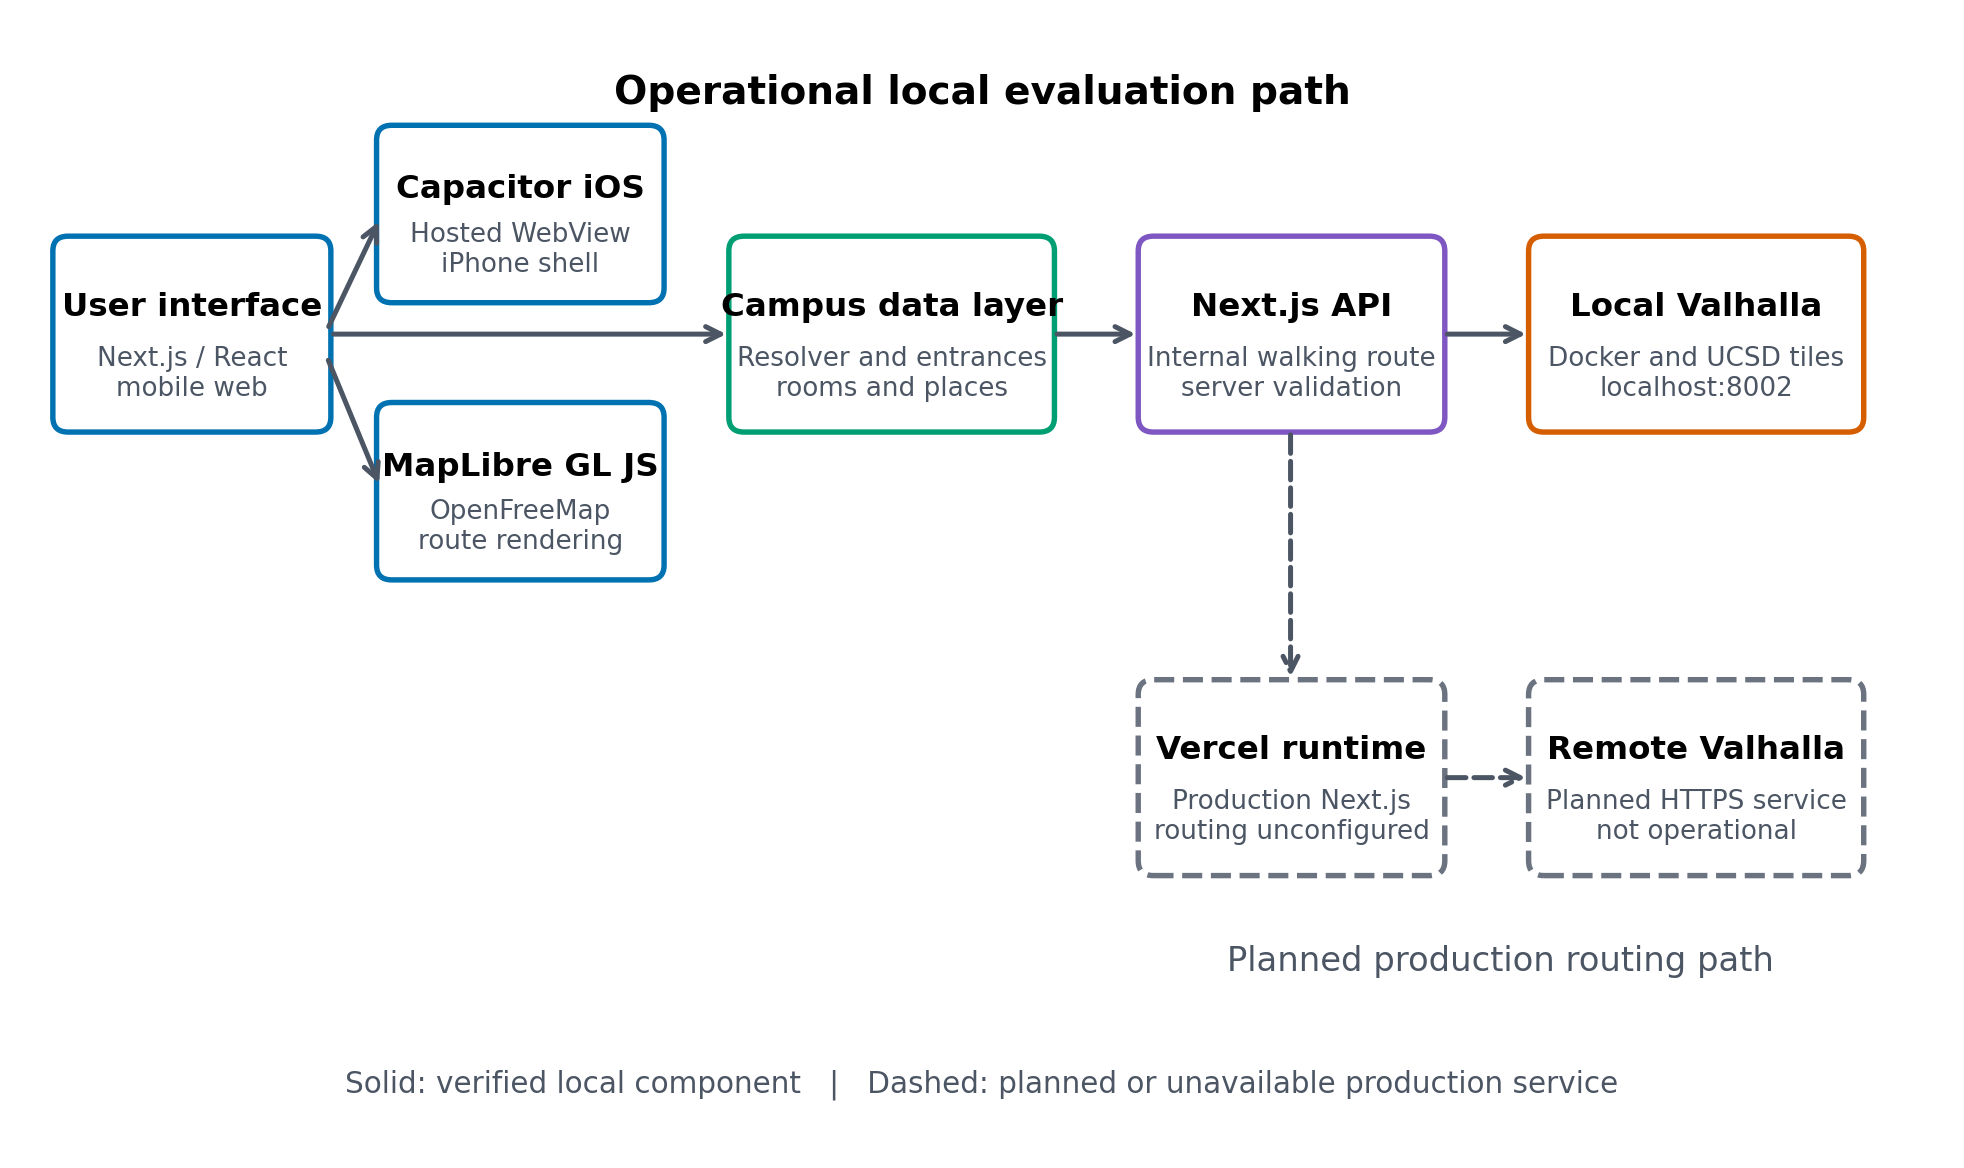
\includegraphics[width=0.86\textwidth]{../figures/figure_07_system_architecture.png}
\caption{Verified TritonNav system architecture. The solid path shows the operational local evaluation stack: Next.js/React interface, Capacitor iOS wrapper, MapLibre/OpenFreeMap visualization, campus resolver, internal walking-route API, and local Docker Valhalla service. Dashed components show the planned production path; remote Valhalla is not operational.}
\label{fig:7}
\end{figure*}
\subsection{Dataset audit and provenance}
The primary dataset is \texttt{TritonNav\_Campus\_Field\_Test\_Workbook.xlsx}. Its SHA-256 digest is \texttt{723d8eb554e628599d5077ab07c8b468205e17f076671aedd52219722b4c006f}. The workbook contains four worksheets: Field Trials, Route Catalog, Issue Log, and Research Dashboard. The analysis script reads the workbook without modifying it and writes cleaned data, tables, figures, and an audit manifest under \texttt{research/}.

The Field Trials sheet contains 41 rows with a Trial ID but only 40 unique identifiers because Trial ID 25 occurs twice. A further row lacks an identifier while containing \texttt{Completed=Yes}; it is excluded from keyed counts. Among keyed records, 39 are marked Yes and two No. The evaluator clarified that completed-but-untimed records are interface/routing checks, not physical walks. One duplicated-ID record remains a documented failed destination-placement check despite its Yes value. The duplicate will be renumbered only in a future source revision.

Timing provenance is divided into four levels. Measured values are numeric entries copied from the source workbook. Calculated values are deterministic transformations, such as end time minus start time or actual minus estimated duration. Normalized values correct an approved representation error while preserving the raw cell. Modeled values come from a current Valhalla snapshot or a stated ratio model and are never called observations.

\subsection{Analysis sets and metrics}
For trial (i), signed timing error is (e\_i=A\_i-V\_i), where (A\_i) is recorded actual time and (V\_i) is Valhalla ETA. Negative error means the recorded walk was faster than the estimate. Absolute error is |(e\_i)|. Because the data contain one evaluator and mostly one observation per route, this report uses descriptive statistics only.

The primary measured-only set contains 23 completed physical-iPhone records with numeric original actual and ETA values. The strict measured set contains 17 of those records for which entered duration agrees with start/end-derived duration within 0.5 minutes. The approved normalized set adds Trial 2 after converting its date-typed value in the ETA-minutes column to the Excel serial value 3.0, producing 24 records. A supplemental timestamp analysis substitutes calculated timestamp durations for seven conflicting entered durations, without changing the workbook or primary results.

The final exploratory set contains 36 records. It combines the 24 normalized records with 12 hypothetical route-model scenarios for untimed interface/routing checks. Each scenario uses a current Valhalla ETA multiplied by 0.875, the median actual-to-ETA ratio in the strict measured subset. The empirical 10th-to-90th percentile ratio range, 0.780 to 1.021, is retained as uncertainty context. Because the same ETA helps generate both the scenario actual and its error, this set cannot independently validate Valhalla. It is included only to test whether a plausible fill strategy overturns the measured descriptive pattern.

Distance was not analyzed. Although workbook headers specify meters, source entries mix decimals, strings labeled in feet, and ambiguous values. GPS accuracy was also excluded because no record contains a numeric meter-valued observation. These omissions avoid false precision.

\section{Experiment}
\subsection{Dataset overview}
Table 1 shows the usable evidence after auditing. The difference between completion status and measured walking trials is substantial: 39 keyed records are marked complete, but only 23 provide original numeric physical-iPhone timing pairs. Fourteen completed records lack both original actual and ETA values, including 12 later approved for hypothetical scenario analysis. The Route Catalog lists six routes under a different identifier convention and no verification dates, and the Issue Log is empty despite narrative problems in Field Trials.

\begin{table*}[t]
\centering
\caption{Descriptive timing results by analysis set.}
\small
\resizebox{\textwidth}{!}{%
\begin{tabular}{lrrrrr}
\toprule
Analysis set & n & Actual mean (min) & ETA mean (min) & Mean signed error (min) & Mean absolute error (min) \\
\midrule
Primary measured-only & 23 & 5.70 & 6.48 & -0.78 & 0.96 \\
Strict measured-only & 17 & 6.06 & 6.82 & -0.76 & 1.00 \\
Exploratory normalized & 24 & 5.58 & 6.33 & -0.75 & 0.92 \\
Timestamp-substituted sensitivity & 24 & 6.75 & 6.33 & 0.42 & 2.33 \\
Exploratory scenario-filled & 36 & 6.40 & 7.28 & -0.88 & 0.99 \\
\bottomrule
\end{tabular}%
}
\end{table*}
\subsection{Measured walking-time agreement}
In the primary measured-only sample, actual walking time averaged 5.70 minutes (median 4.0, standard deviation 4.12), while Valhalla ETA averaged 6.48 minutes (median 6.0). Mean signed error was -0.78 minutes, median signed error was -1.0 minute, and mean absolute error was 0.96 minutes. Errors ranged from -4 to +1 minute. Thus, in this small dataset, Valhalla generally estimated slightly longer walks than were recorded.

The strict 17-trial subset is important because it removes records with conflicting duration fields. It produced nearly the same mean signed error (-0.76 minutes) and a mean absolute error of 1.00 minute. This consistency suggests that the central descriptive result is not created solely by the moderate timestamp conflicts. Figure 1 visualizes the agreement and separates timestamp-consistent records from conflicts. Trial 2's approved 3.0-minute ETA normalization is shown as an open diamond and remains outside the measured-only sample.

\begin{figure*}[t]
\centering
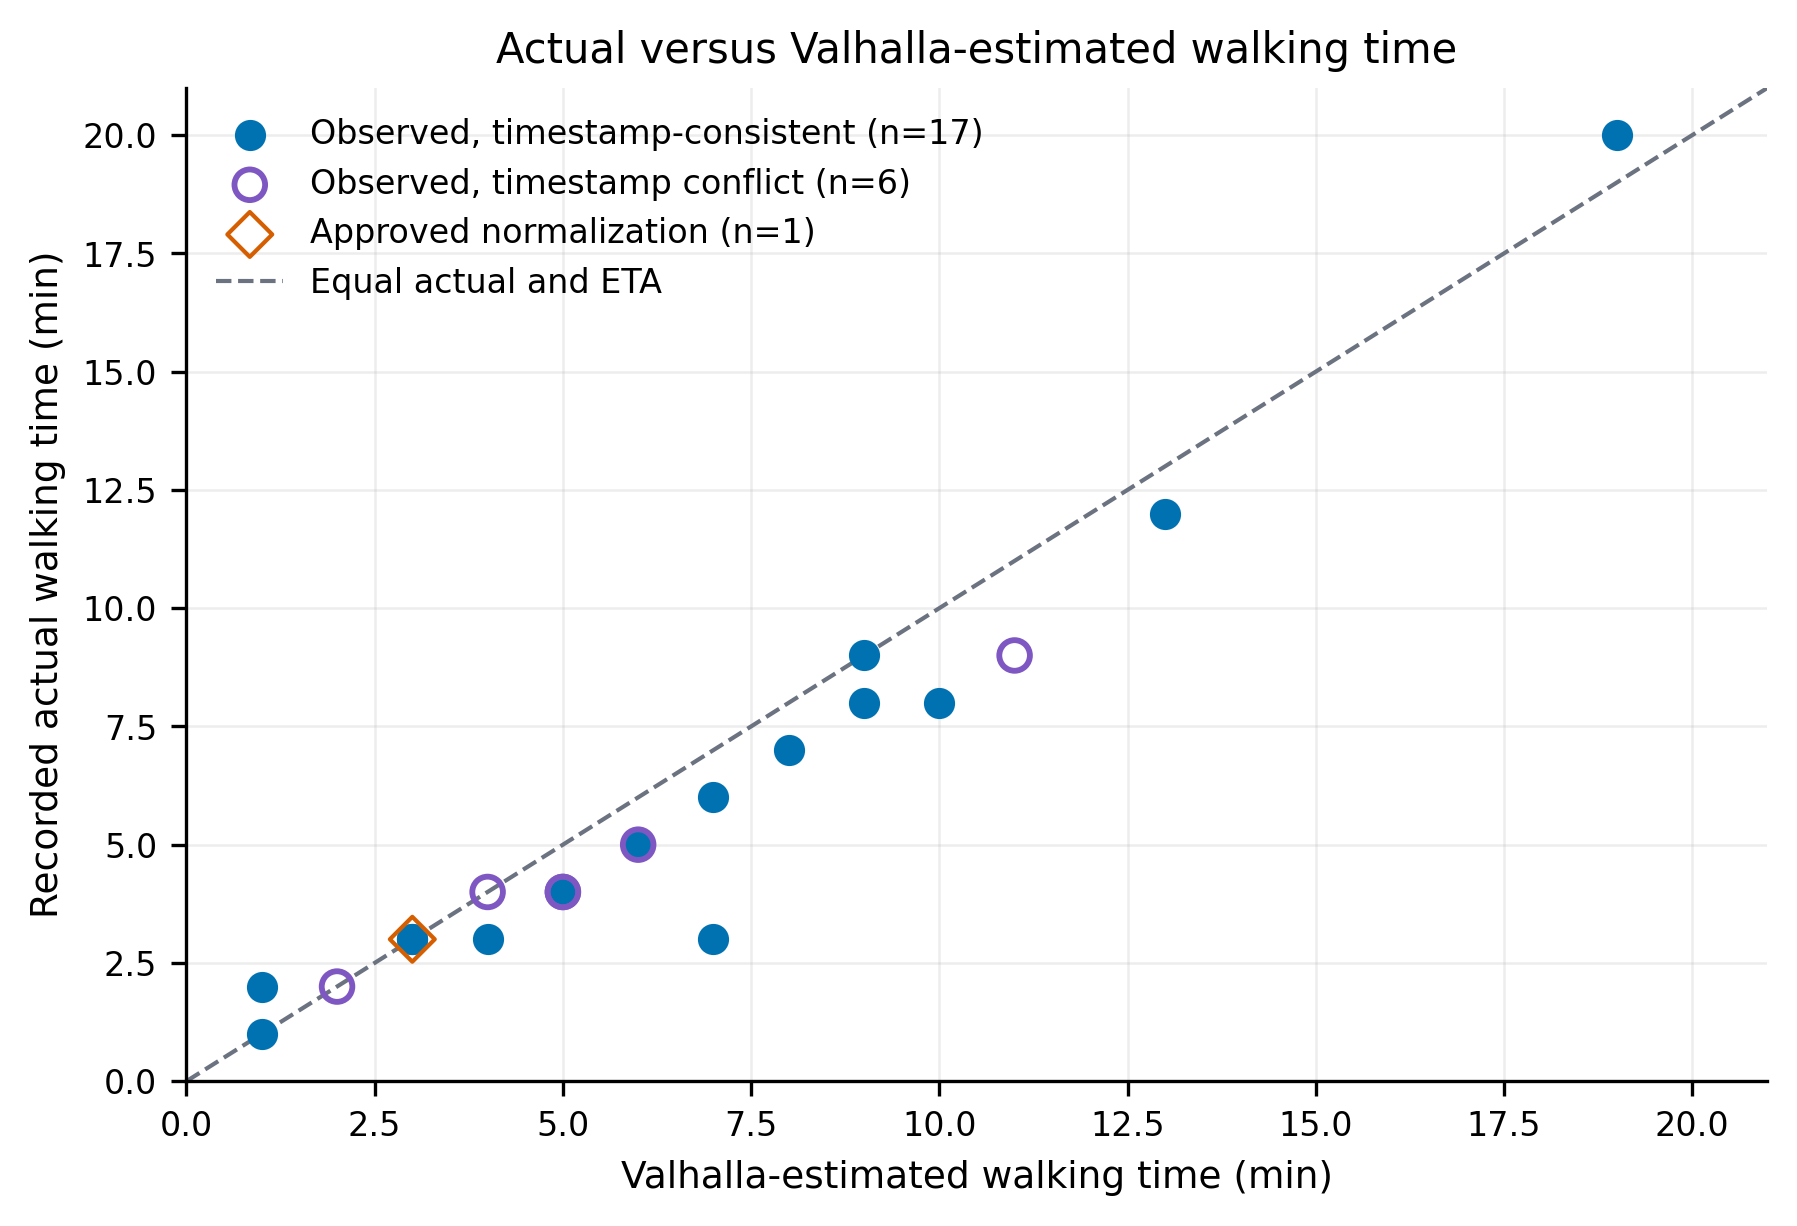
\includegraphics[width=0.86\textwidth]{../figures/figure_01_actual_vs_valhalla.png}
\caption{Actual versus Valhalla-estimated walking time. Recorded physical-iPhone observations are separated by timestamp consistency. The dashed line denotes equality. The open diamond is the approved Trial 2 normalization and is excluded from the primary measured-only sample.}
\label{fig:1}
\end{figure*}
The result is not a calibrated accuracy guarantee. Routes differ in length, most identifiers appear once, the evaluator is constant, timing is coarse, and no numeric GPS accuracy is available. Figure 6 therefore presents descriptive route pairs rather than nonexistent repeats.

\begin{figure*}[t]
\centering
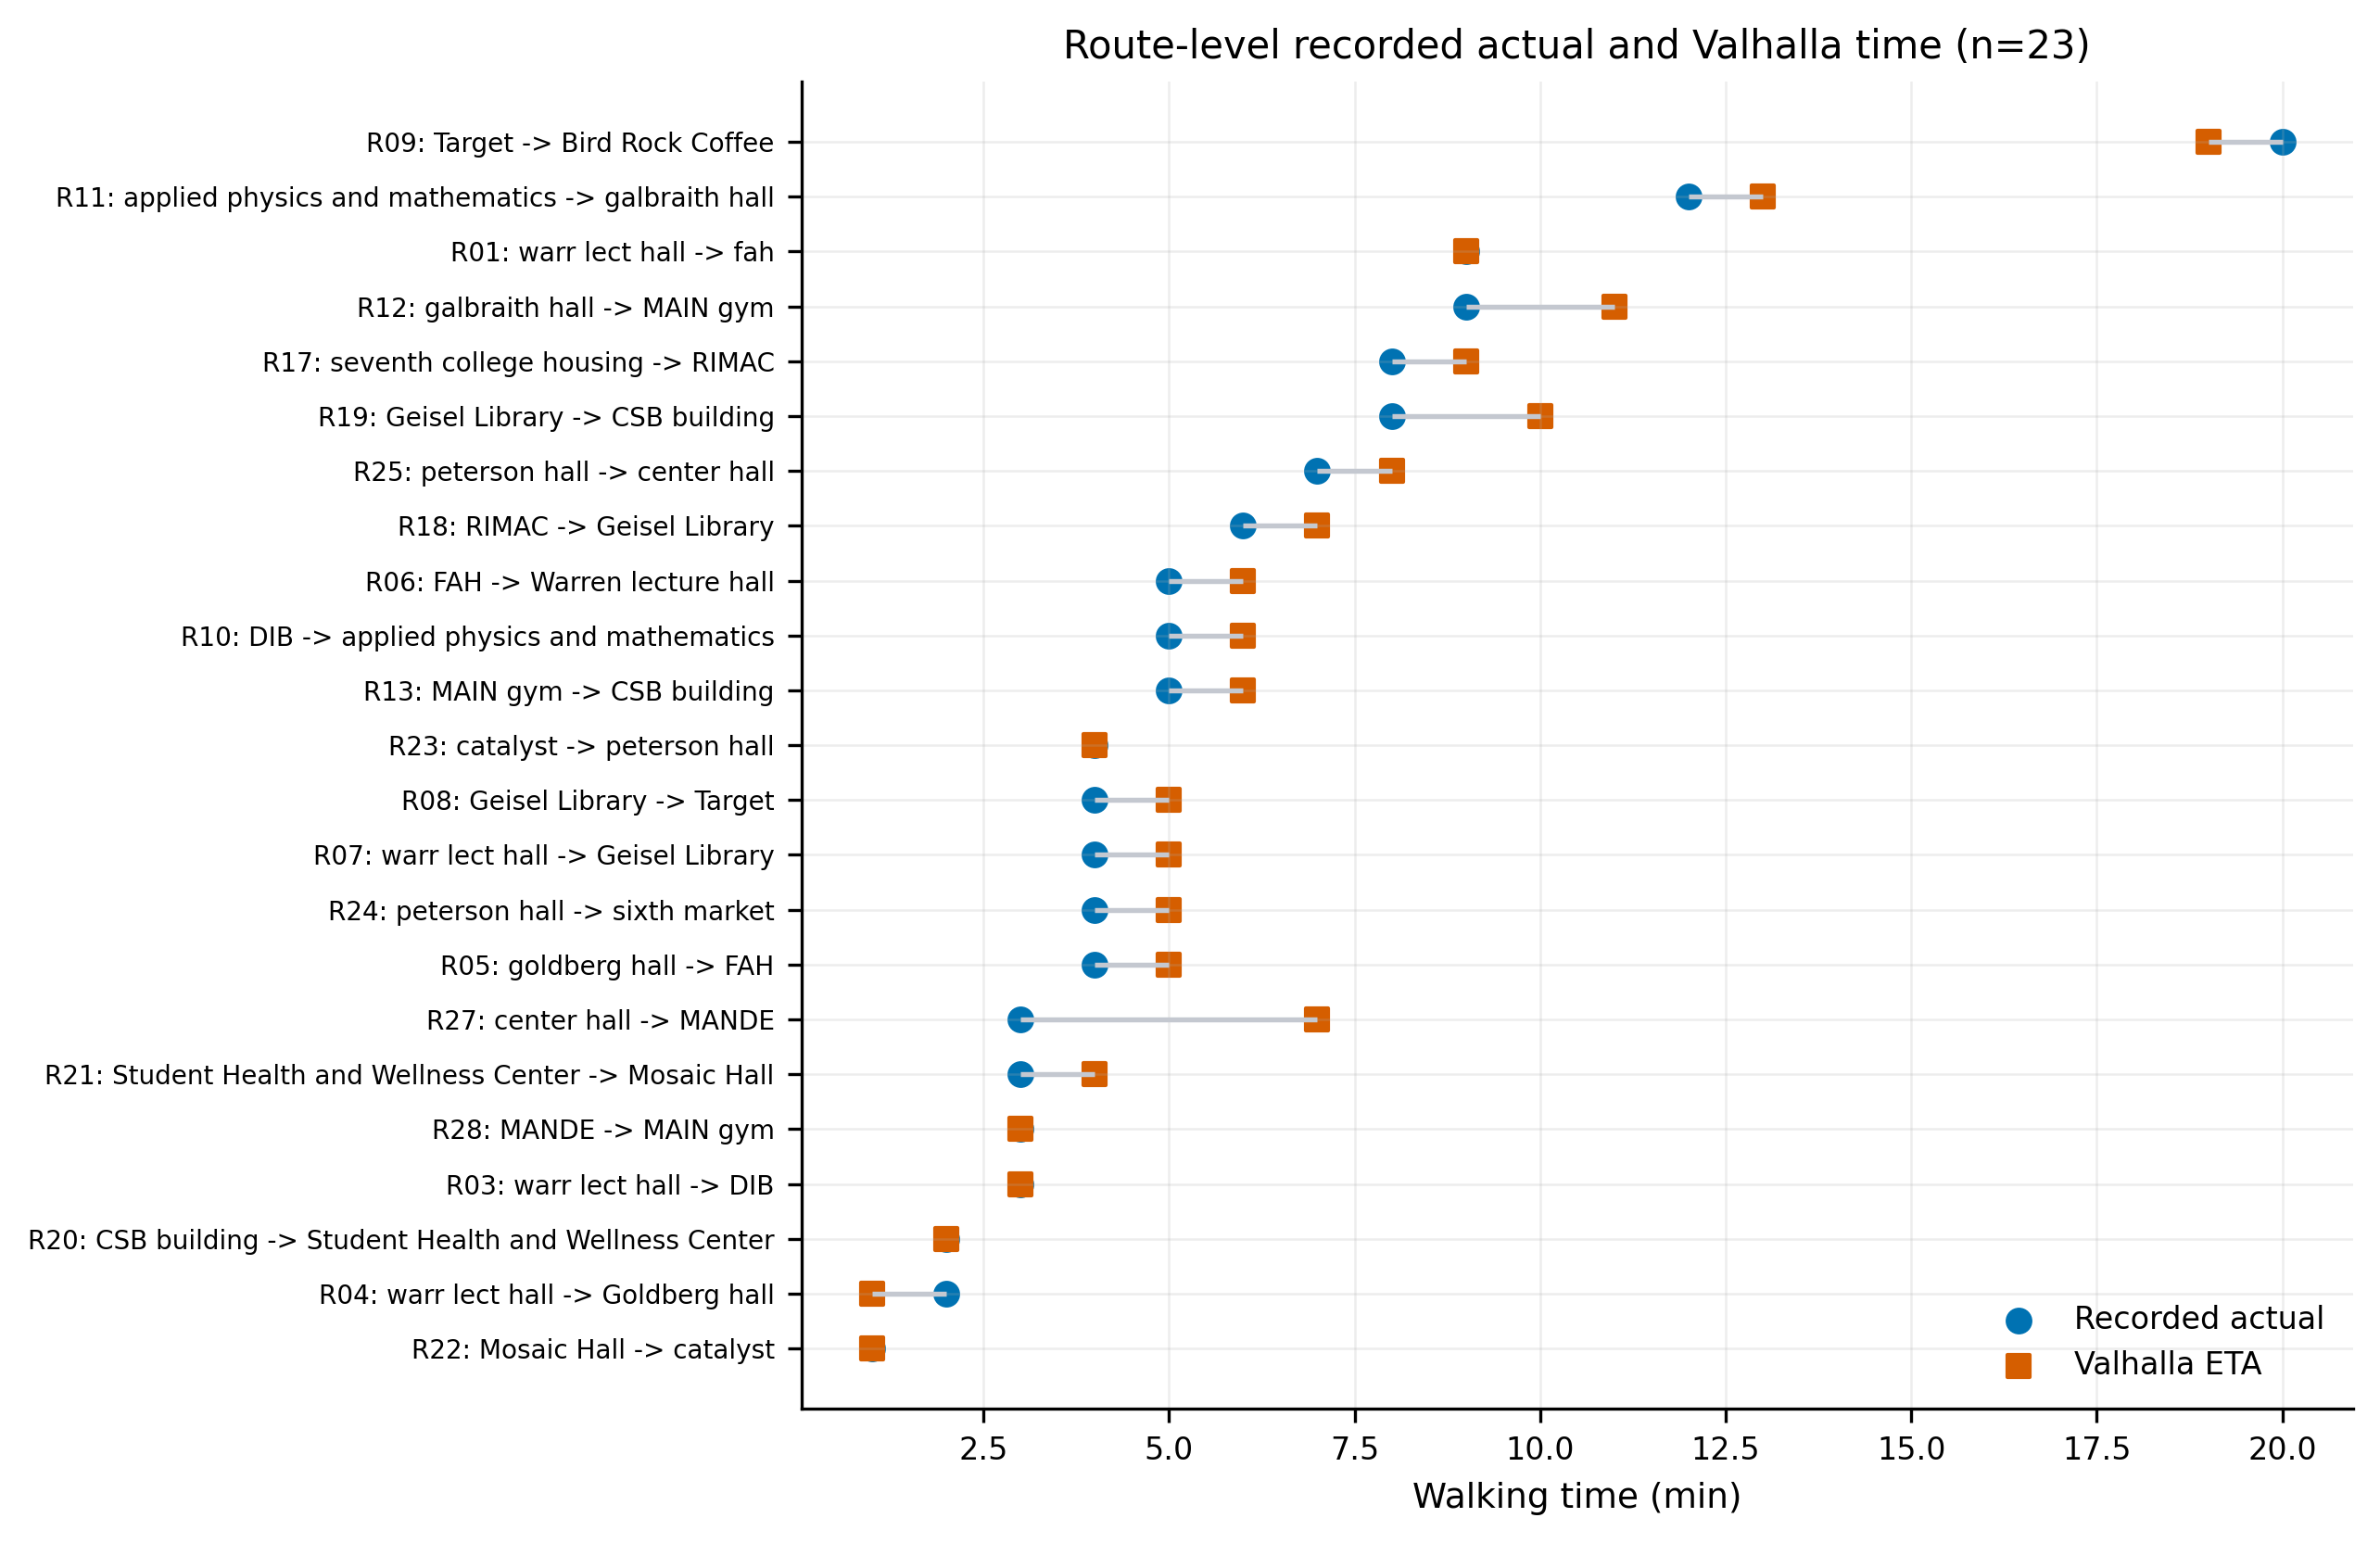
\includegraphics[width=0.86\textwidth]{../figures/figure_06_route_level_performance.png}
\caption{Route-level recorded and estimated walking time. Dumbbells compare recorded actual time with Valhalla ETA for each eligible physical-iPhone record. Route IDs are unique in the workbook, so the figure does not estimate within-route repeatability.}
\label{fig:6}
\end{figure*}
\subsection{Routing and destination outcomes}
Two records are marked incomplete. The CSB Building to Marshall College check returned no route and reportedly displayed a college diagram; the RIMAC to Seventh College Housing check returned neither a route line nor a map. Current resolver diagnostics also cannot resolve both endpoints for those historical labels, so these records identify destination-data gaps as well as route failures.

The workbook records additional destination problems. Peterson Hall to Sixth Market reportedly placed the market near DIB. The duplicated Trial ID 25 record for Center Hall to Pepper Canyon Hall reported four wrong turns, an incorrect entrance, and placement at Bonner Hall. These examples matter because a correct routing engine cannot compensate for an incorrect destination anchor. They support TritonNav's architectural decision to resolve rooms, buildings, and entrances before invoking Valhalla.

Figure 5 aggregates issue indicators without treating categories as mutually exclusive. Eight records report at least one wrong turn, four contain narrative issues, two are routing failures, and two describe incorrect destination placement. One record marks the entrance incorrect, one marks the route line not visible, and one marks the map not loaded. The bars cannot be summed into a unique number of affected trials because one record may contribute to several categories.

\begin{figure*}[t]
\centering
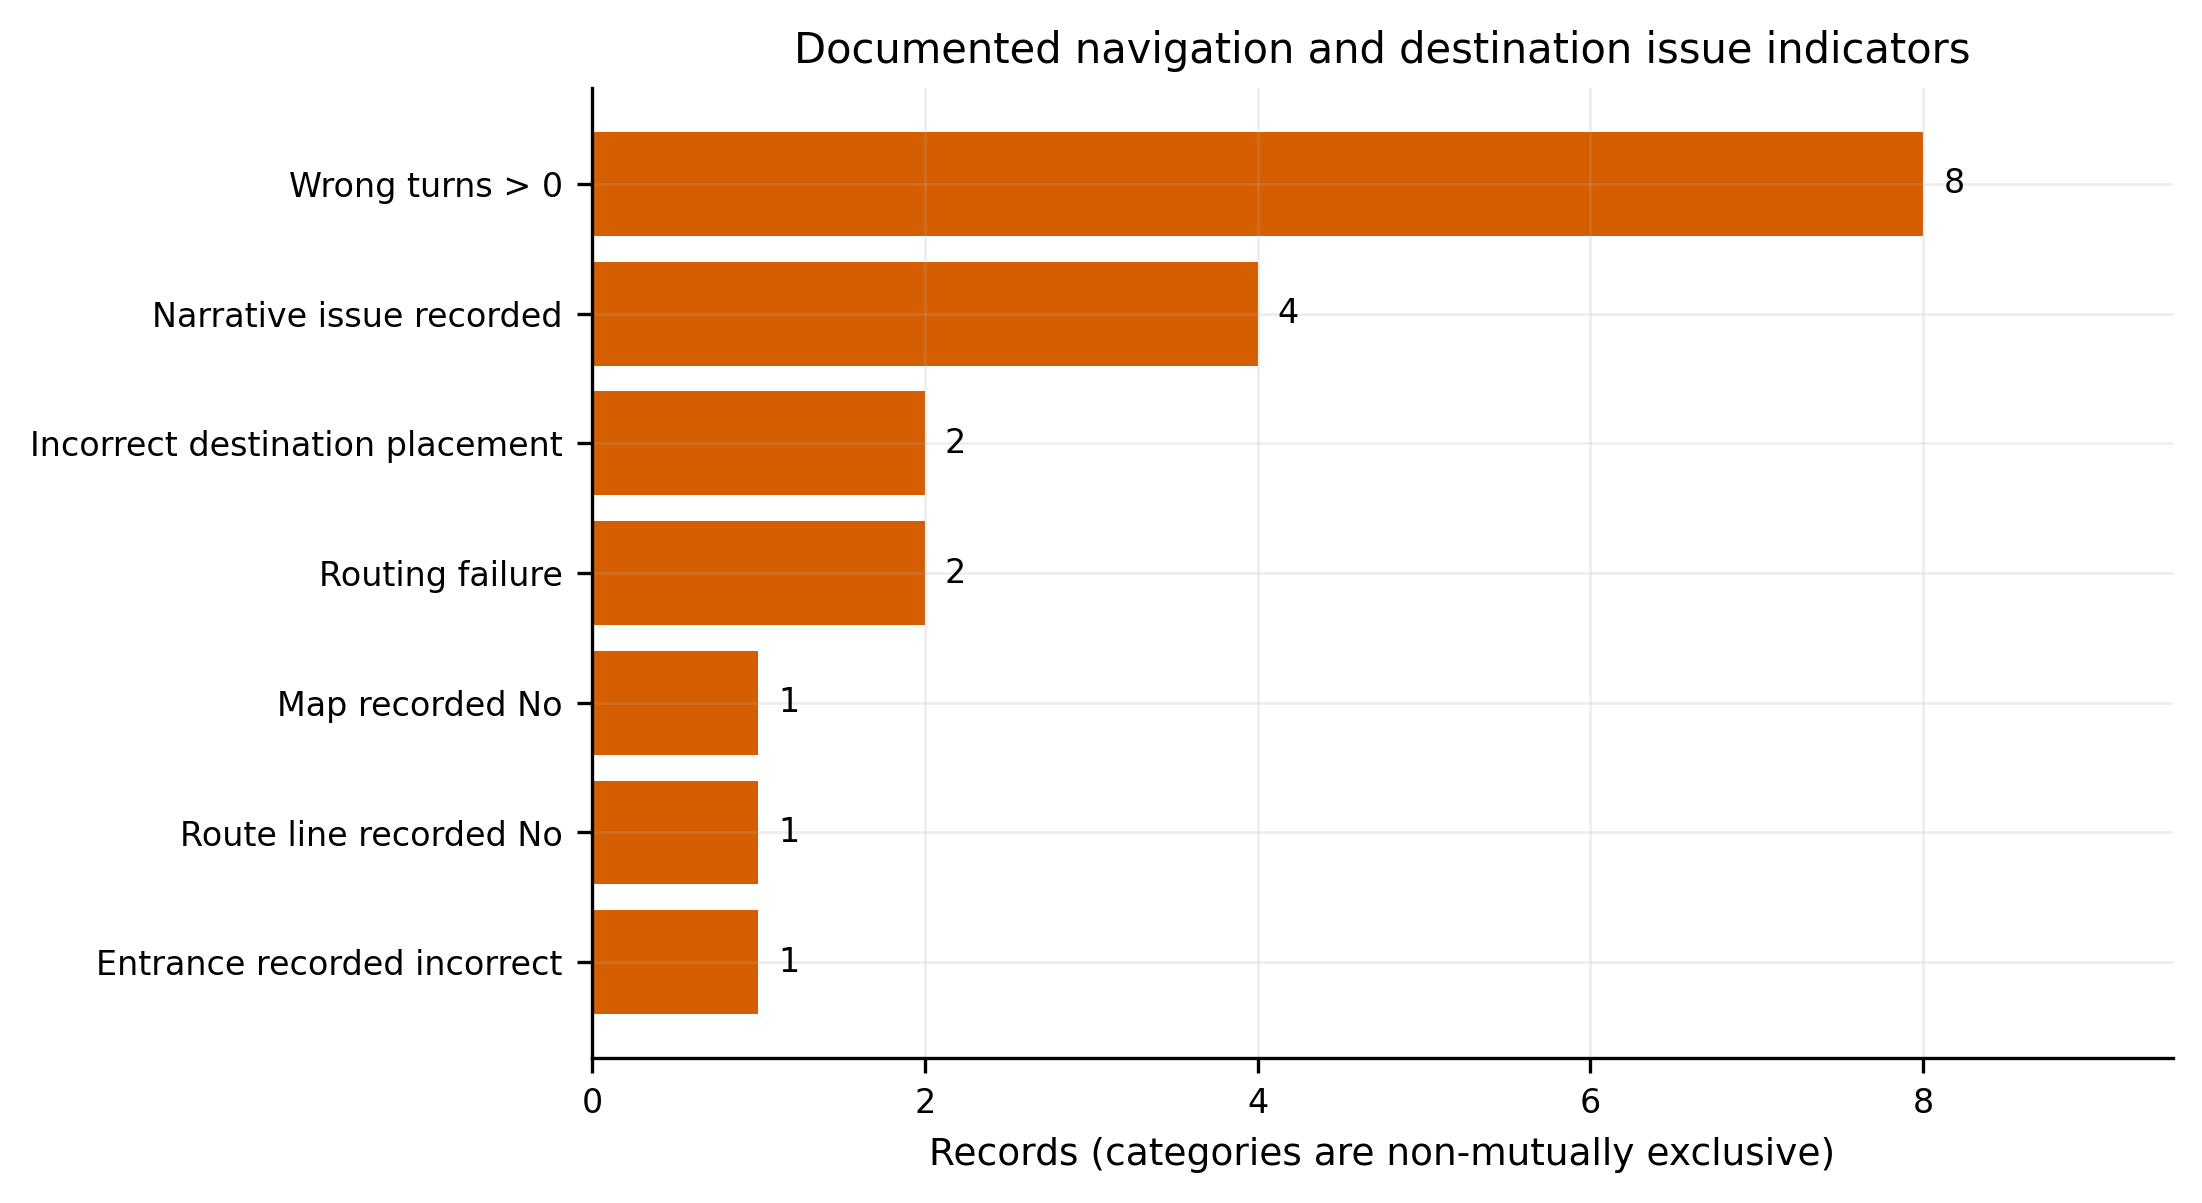
\includegraphics[width=0.86\textwidth]{../figures/figure_05_navigation_issues.png}
\caption{Navigation and destination issue indicators. Counts come from structured workbook fields and written observations. Categories overlap and must not be summed as a total number of affected trials.}
\label{fig:5}
\end{figure*}
The Yes labels provide heterogeneous interface evidence. The 12 untimed iPhone rows used in scenarios indicate successful interface/routing checks, not walking durations. The Mac check likewise demonstrates service behavior rather than a traversal. This prevents a rendering success from being promoted into a mobility outcome.

\subsection{Sensitivity analyses}
The approved Trial 2 normalization changes the primary descriptive statistics only slightly when added to the exploratory normalized set: mean signed error becomes -0.75 minutes and mean absolute error 0.92 minutes. The 12 scenario-filled records also leave the direction and scale similar, with mean signed error -0.88 minutes and mean absolute error 0.99 minutes. This apparent stability must be interpreted cautiously because the scenario actual values are mechanically derived from Valhalla ETA using a measured-sample ratio.

The timestamp-derived sensitivity analysis demonstrates why source review matters. Seven records have a conflict greater than 0.5 minutes, including Trial 23, whose entered actual duration is 4 minutes while its timestamps span 33 minutes. Substituting all seven timestamp-derived values changes mean signed error from -0.75 to +0.42 minutes and increases mean absolute error from 0.92 to 2.33 minutes. The median signed error remains -1.0 minute, revealing that one extreme discrepancy drives much of the mean shift. The timestamps are therefore reported as supplemental alternatives rather than replacements. Trial 23 should be reconciled against contemporaneous notes before either value supports a future claim.

\subsection{Limitations and next experiment}
The largest limitation is experimental design, not routing code. One evaluator cannot represent the variability of campus users, mobility needs, walking speeds, or device conditions. Unique routes prevent repeatability estimates. Minute-level timing is coarse, GPS accuracy is absent, distances are unusable until units are normalized, and app version metadata are incomplete. The workbook dashboard also overcounts completed records by including a blank-ID row, and the empty Issue Log weakens traceability.

A stronger follow-up should pre-register a compact set of repeated routes, recruit multiple participants, capture precise timestamps and horizontal location accuracy, and separate interface checks from walked trials at collection time. Each trial should store a canonical route ID, application commit, device and OS, origin and destination entity IDs, selected entrance, provider response metadata, and a linked issue record. Accessibility claims should wait for verified UCSD GIS data and evaluation with representative users. The existing architecture can support that study, but the current evidence cannot substitute for it.

\section{Conclusion}
TritonNav demonstrates that a campus-specific destination resolver, a server-side Valhalla adapter, and MapLibre route rendering can operate as a coherent mobile prototype. In 23 measured physical-iPhone trials, recorded walks were descriptively about 0.78 minutes shorter than Valhalla estimates on average, with mean absolute error near one minute. A strict timestamp-consistent subset produced a similar result. Field observations nevertheless exposed two route failures, destination-placement errors, entrance problems, and data-governance weaknesses that are central to campus navigation quality.

The approved sensitivity analyses do not alter the main conclusion, but they clarify its uncertainty. The Trial 2 normalization and 12 hypothetical route-model scenarios preserve the general measured pattern; timestamp substitution is highly sensitive to one 29-minute discrepancy. The correct next step is therefore not a stronger accuracy claim. It is a controlled, multi-participant study built on verified campus coordinates, explicit entrance provenance, repeated routes, precise timing, and structured issue logging. TritonNav's modular design makes that progression possible while preserving truthful behavior when routing or destination data are unavailable.

\begin{thebibliography}{9}
\bibitem{ref1} R. Tahir and J. Krogstie. "Impact of Navigation Aid and Spatial Ability Skills on Wayfinding Performance and Workload in Indoor-Outdoor Campus Navigation: Challenges and Design." \textit{Applied Sciences}, 13(17):9508, 2023. \url{https://doi.org/10.3390/app13179508}
\bibitem{ref2} C. Prandi, B. R. Barricelli, S. Mirri, and D. Fogli. "Accessible wayfinding and navigation: a systematic mapping study." \textit{Universal Access in the Information Society}, 22(1):185-212, 2023. Published online 2021. \url{https://doi.org/10.1007/s10209-021-00843-x}
\bibitem{ref3} M. Haklay and P. Weber. "OpenStreetMap: User-Generated Street Maps." \textit{IEEE Pervasive Computing}, 7(4):12-18, 2008. \url{https://doi.org/10.1109/MPRV.2008.80}
\bibitem{ref4} MapLibre contributors. "MapLibre GL JS Documentation." \url{https://maplibre.org/maplibre-gl-js/docs/} (accessed September 30, 2026).
\bibitem{ref5} Valhalla contributors. "Valhalla Documentation: HTTP API and Routing Architecture." \url{https://valhalla.github.io/valhalla/api/} (accessed September 30, 2026).
\bibitem{ref6} H. Butler, M. Daly, A. Doyle, S. Gillies, S. Hagen, and T. Schaub. "The GeoJSON Format." RFC 7946, Internet Engineering Task Force, 2016. \url{https://www.rfc-editor.org/rfc/rfc7946}
\bibitem{ref7} Ionic. "Capacitor: Cross-platform Native Runtime for Web Apps." \url{https://capacitorjs.com/docs} (accessed September 30, 2026).
\bibitem{ref8} OpenFreeMap. "OpenFreeMap Documentation and Attribution." \url{https://openfreemap.org/} (accessed September 30, 2026).
\bibitem{ref9} Vercel. "Next.js Route Handlers." \url{https://nextjs.org/docs/app/getting-started/route-handlers} (accessed September 30, 2026).
\end{thebibliography}
\end{document}
